\documentclass{article}
\usepackage[final]{neurips_2024}

\usepackage[utf8]{inputenc} % allow utf-8 input
\usepackage[T1]{fontenc}    % use 8-bit T1 fonts
\usepackage{hyperref}       % hyperlinks
\usepackage{url}            % simple URL typesetting
\usepackage{booktabs}       % professional-quality tables
\usepackage{amsfonts}       % blackboard math symbols
\usepackage{nicefrac}       % compact symbols for 1/2, etc.
\usepackage{microtype}      % microtypography
\usepackage{xcolor}         % colors

\usepackage{graphicx}
\usepackage{float}

\title{Homework 2}

\author{
  Kevin Lei \\
  Department of Computer Science and Engineering \\
  Texas A\&M University \\
  College Station, TX 77843 \\
  \texttt{kevinlei@tamu.edu} \\
}

\begin{document}
\maketitle

\section{Tweaking Epoch Count and Learning Rate}

The following are the decision boundaries plotted with the training data for variations on epoch and learning rate.

\begin{minipage}{0.5\textwidth}
  \begin{figure}[H]
    \centering
    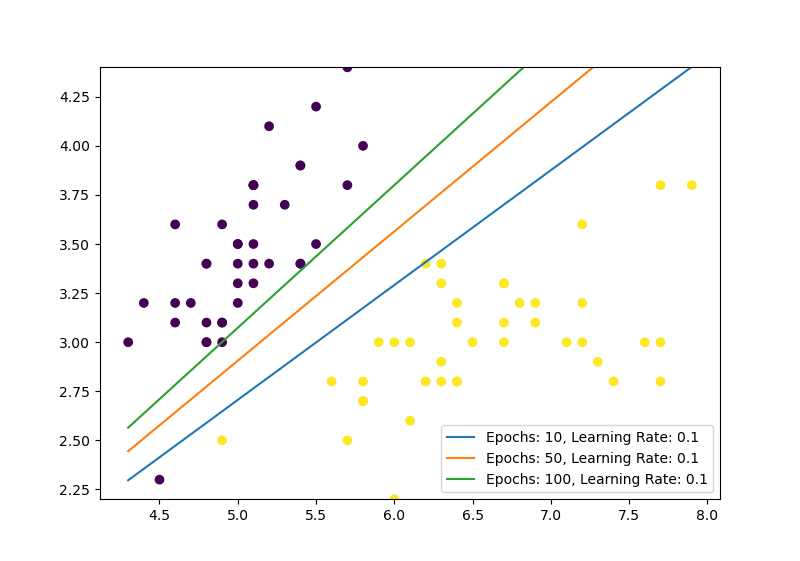
\includegraphics[width=\linewidth]{Figure_1.png}
    \caption{Perceptron with variable epochs.}
  \end{figure}
\end{minipage}
\begin{minipage}{0.5\textwidth}
  \begin{figure}[H]
    \centering
    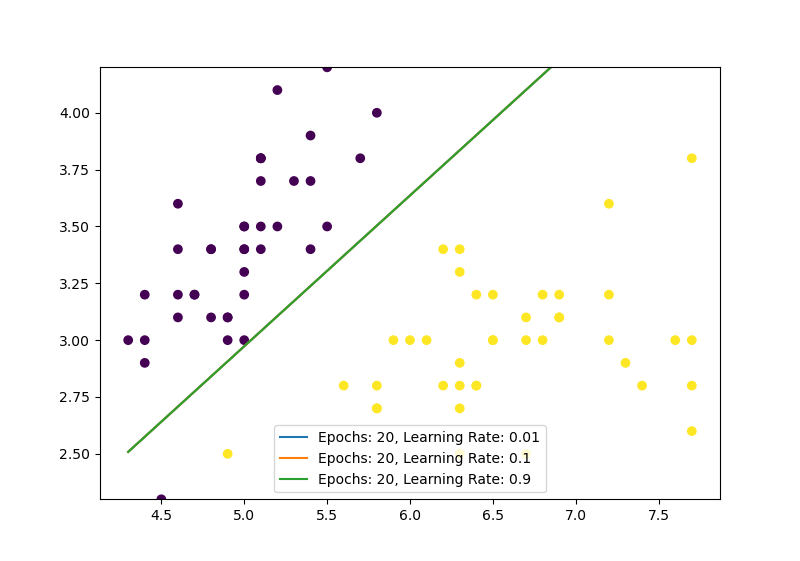
\includegraphics[width=\linewidth]{Figure_2.png}
    \caption{Perceptron with variable learning rate.}
  \end{figure}
\end{minipage}

As we can see from Figure 1, having a suboptimal number of epochs can lead to a decision boundary that does not accurately separate the two classes.
Compared to the initial settings (1000 epochs and 0.01 learning rate), the decision boundaries produced by 10, 50, and 100 epochs are not as accurate.
Additionally, notice that the decision boundary produced by 50 epochs seems to have the best margin of separation between the two classes, compared to the other epoch values.
This suggests that for a fixed learning rate, having too many or too few epochs can lead to a suboptimal decision boundary.
Theoretically, less epochs would lead to a decision boundary that is not as accurate, while more epochs would lead to a decision boundary that is overfit to the training data.

Speaking in terms of learning rate, Figure 2 shows that changing the learning rate between 0.01, 0.1, and 0.9 does not produce significant differences in the decision boundary.
However, that is not to say that leraning rate is generally not an important hyperparameter.
For more complex datasets, we may see a more significant impact of learning rate on the decision boundary.

\newpage

\section{Error Accumulation}

The following is a graph of the accumulated number of misclassifications over all the epochs for the perceptron algorithm.

\begin{figure}[H]
  \centering
  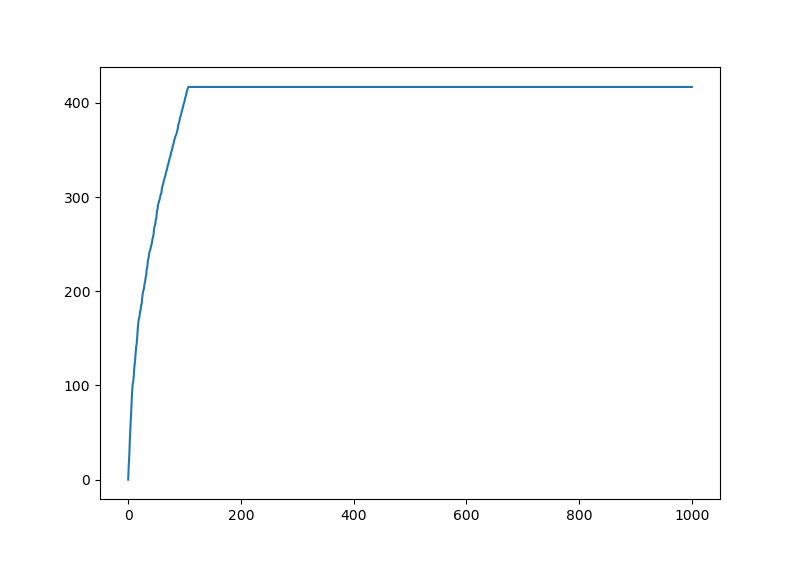
\includegraphics[width=0.65\linewidth]{Figure_3.png}
  \caption{Accumulated number of misclassifications over all epochs.}
\end{figure}

As we can see from the graph, the number of misclassifications converges to a value slightly over 400 after about 100 epochs with a learning rate of 0.01.
Also, the rate of change in the number of misclassifications decreases as the number of epochs increases.
This suggests that the perceptron algorithm is converging to a solution that is not perfect, but is close to the optimal solution.

\section{Linearly Inseparable Data}

Using Versicolor instead of Setosa, the following is the decision boundary plotted with the training data.

\begin{figure}[H]
  \centering
  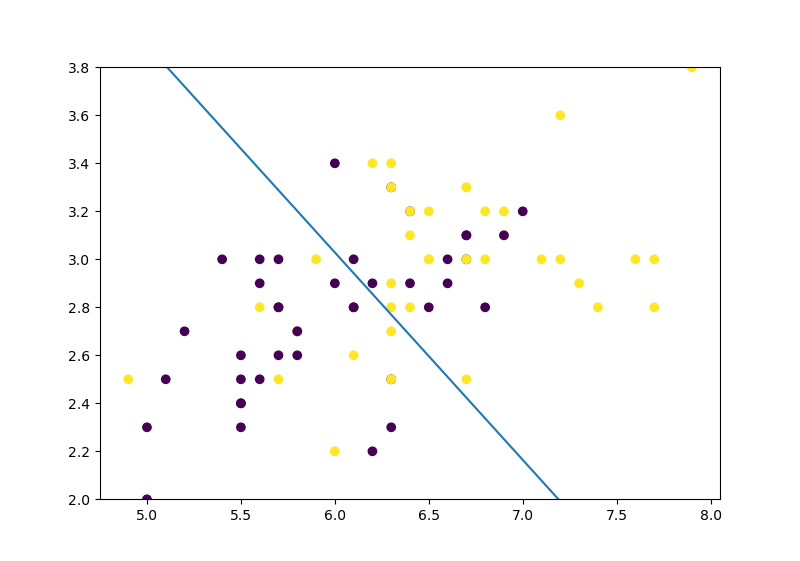
\includegraphics[width=0.65\linewidth]{Figure_4.png}
  \caption{Perceptron with Versicolor instead of Setosa.}
\end{figure}

As we can see from the graph, the perceptron algorithm is unable to converge to a solution that separates the two classes due to the fact that there is no linear decision boundary that can separate the two classes.
The points seem to be scattered within each other, which makes it impossible for a single perceptron to separate the two classes.

\end{document}